% Instructions to change to html version:
% Comment out:
%  minipage, multicols,columnbreak, mathbf, hrule
% Replace all: \begin{minipage}% \end{minipage} %\begin{multicols}  %\end{multicols}  %\columnbreak %% \begin{framed} %\end{framed} %%\hrule
% Replace \mathbf with \boldsymbol
% Replace $$ with \[ or \]and $ with \( or \)
% Enclose graphics in figure environments and add captions
% 			search \includegraphics
% Re-tag \df environments as sections, subsections, etc.
% Command Line Code to Create html version:
%First: pdflatex -shell-escape filename.tex                                   
%Second, for each figure: inkscape "filename-figure1.pdf" -o "filename-figure1.png"
% Third: htlatex filename.tex "ht5mjlatex.cfg, charset=utf-8" " -cunihtf -utf8"

\documentclass[10pt]{article}

%\usepackage{tikz, pgf,pgfplots,wasysym,array}
%\usepackage{wasysym,array}

\usepackage{amsmath,amssymb}

\ifdefined\HCode
  \def\pgfsysdriver{pgfsys-tex4ht-updated.def}
\fi 
%\ifdefined\HCode
%  \def\pgfsysdriver{pgfsys-dvisvgm4ht.def}
%\fi 
\usepackage{tikz}
\usetikzlibrary{calc,decorations.markings,arrows}
\usepackage{pgfplots}

\pgfplotsset{compat=1.12}
\usepackage{myexternalize}
\usetikzlibrary{calc,decorations.markings,arrows}
\usepackage{framed}
\usepackage[none]{hyphenat}

\input{../../../common/1336_header_test.tex}
\begin{document}

\everymath{\displaystyle}


\newcommand{\ihat}{\boldsymbol{\hat{\textbf{\i}}}}
\newcommand{\jhat}{\boldsymbol{\hat{\textbf{\j}}}}
\newcommand{\khat}{\boldsymbol{\hat{\textbf{k}}}}

\let\oldvec\vec
\renewcommand{\vec}[1]{\oldvec{\boldsymbol{#1}}}

\renewcommand{\u}{\vec{u}}
\renewcommand{\v}{\vec{v}}
\newcommand{\w}{\vec{w}}
\renewcommand{\r}{\vec{r}}
\renewcommand{\a}{\vec{a}}
\renewcommand{\b}{\vec{b}}
\newcommand{\n}{\vec{n}}

\newcommand{\<}{\left\langle}
\renewcommand{\>}{\right\rangle}

\renewcommand{\myTitle}{MATH 1336: Calculus III}

\renewcommand{\mySubTitle}{Section 2.5, Part 2: Planes \vspace*{-.2in}}
%~\hfill Name: \underline{~~~~~~~~~~~~~~~~~~~~~~~~~~~~~~~~~~~~~~~~~~~~~~~}

\lectTitle{\vspace*{-.5in}\myTitle}{\vspace*{.1in}\mySubTitle \vspace*{-.1in}}


\setlength{\columnseprule}{0.4pt}
\setlength{\columnsep}{3em}

%\hspace*{-.8in}%\begin{minipage}{1.25\textwidth}
%\begin{framed}


\section*{Equations of Planes:}
You may have geometric intuition that three points determine a plane. Our equations for planes will be built using one point, \(P_0\), and vector that is perpendicular to the plane, called the normal vector: \(\n\). 

%\begin{minipage}{.4\textwidth}


\begin{figure}[!h]
\centering
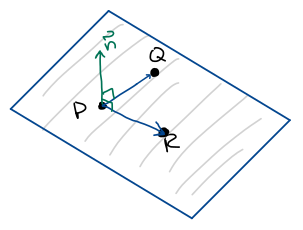
\includegraphics[height=1.25in]{Ch2s5-planes2a.png}
\caption{Illustration of a plane containing two vectors, and a vector that is perpendicular to the plane.}
\end{figure}

%\end{minipage}
\hspace*{.2in}
%\begin{minipage}{.5\textwidth}

Note that if we have three points that are on the plane, \(P, Q, R\), we can find the normal direction by taking the cross product of vectors drawn from one point to the other two points, for example: \(\n = \overrightarrow{PR} \times \overrightarrow{PQ}\).

%\end{minipage}

The plane equations are built on two key ideas: the normal vector, \(\n \), is perpendicular to any vector that lies in the plane, and that the dot product of two perpendicular vectors is zero.\\


Let \(\vec{r}_0 = \<x_0, y_0, z_0\>\) be the position vector for a specific point on the plane, \(P_0  = (x_0, y_0, z_0)\), and let \(\vec{r} = \< x, y, z\>\) be the position vector for any general point on the plane: \(P = ( x, y, z)\). Then the vector \(\overrightarrow{P_0 P} = \r - \r_0 = \< x - x_0, y - y_0, z-z_0\>\) lies in the plane.
Finally, let \(\n = \<a, b, c\>\) be the normal vector.  Then the plane can be described by any of the following types of equations:\\

%\begin{minipage}{.4\textwidth}


\begin{figure}[!h]
\centering
%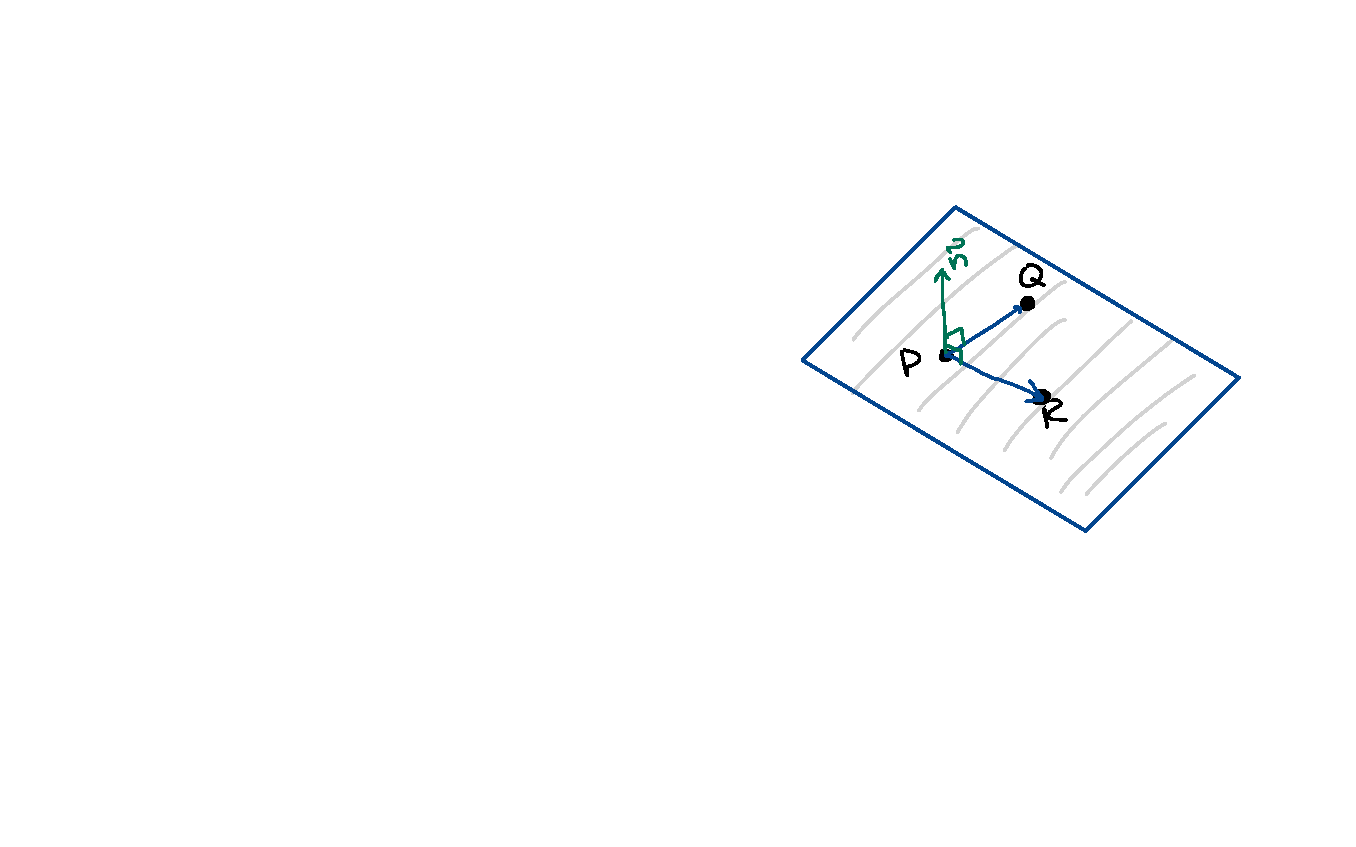
\includegraphics[height=1.25in]{Ch10s5-planes2a.pdf}
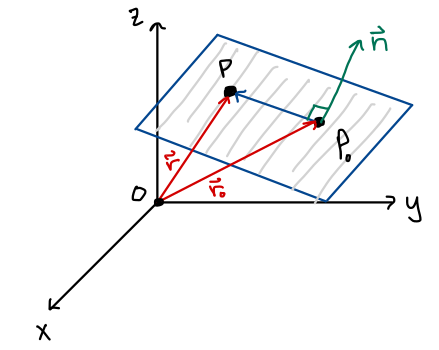
\includegraphics[width=\textwidth]{Ch2s5-planes2b.png}
\caption{Illustration of a plane in three dimensions for reference when building plane equations.}
\end{figure}

%\end{minipage}
\hspace*{.2in}
%\begin{minipage}{.5\textwidth}





\textbf{Vector Equation:}

\[
\n \cdot (\r- \r_0) = 0
\]
~\\

\textbf{Scalar Equation:}

\[
a(x-x_0) + b(y-y_0) + c(z-z_0) = 0
\]

~\\

\textbf{Standard Form:}\\

\[
ax + by + cz +d = 0
\]

~\\

%\end{minipage}

Note that \(a, b, c\) are sometimes called the \textbf{attitude numbers} of the plane.

%\end{framed}
%\end{minipage}



\section*{Warmup: Parallel, Perpendicular, or Neither?}
For each of the following, determine whether the given items are parallel, perpendicular, or neither:
\newcounter{prob}


\begin{list}{\bf{Warmup \arabic {prob}: }}{\usecounter{prob}}

\item The vectors:
\[ 
\v_1 = < 1, 2, 3>, \qquad \v_2 = 3\ihat - 2\jhat + \frac{2}{3}\khat
\]

\vfill

\item The lines:
\begin{eqnarray*}
L_1: \quad  \frac{x-17}{5} = \frac{y-4}{2} = \frac{z-15}{6}  \qquad \qquad%\\
L_2: \quad  \frac{x+10}{6} = \frac{y+10}{4} = \frac{z+21}{9}
\end{eqnarray*}


\vfill


%\item The plane with the standard equation \(2x-y-5z = 0\) and each of the planes listed below:
%\begin{eqnarray*}
%-6x + 3y + 15z &=& 3\\
%x+2y &=& -4\\
%2x - 5z &=& -1
%\end{eqnarray*}
%
%\vfill

%
%\item The line with vector equation \(\r(t) = <5-3t, 2+4t, 4-2t>\) and each of the planes listed below:
%\begin{eqnarray*}
%-4.5x+6y-3z &=& -21\\
%3x + 5y - 2z &=& -30\\
%2x + 2y - 3z &=& 11\\
%4x + 7y + 8z &=& 11
%\end{eqnarray*}
%
%\vfill




\end{list}



\pagebreak

\section*{Example 3:}% (Pre-class Video):} 

Find the equation of the plane that passes through 

\[P = (3,0,0), \quad Q = (0, 2, 0), \quad R = (0,0,1)\]

\hrule
\vspace*{.1in}

%In the video, I 
Let's choose to build \(\n\) using the vectors \(\overrightarrow{PQ}\) and \(\overrightarrow{PR}\), and to use \(P\) to define \(\r_0\). Different choices would result in equations for the plane that might look slightly different, but would still describe the same plane!


\[
\n = \overrightarrow{PQ} \times \overrightarrow{PR} = \begin{vmatrix}
\ihat & \jhat & \khat\\
-3 & 2 & 0\\
-3 & 0 & 1
\end{vmatrix}
 = \begin{vmatrix}
 2 & 0\\
 0 & 1
 \end{vmatrix}
 \ihat
 - \begin{vmatrix}
 -3 & 0\\
 -3 & 1
 \end{vmatrix}
 \jhat
 + \begin{vmatrix}
 -3 & 2\\
 -3 & 0
 \end{vmatrix}
 \khat
 = (2-0)\ \ihat - (-3-0)\ \jhat + (0+6)\ \khat = 2\ \ihat + 3\ \jhat + 6\ \khat
 \]
 
  \[
\n = \<2, 3, 6\>, \qquad \r_0 = \<3, 0, 0\>
\]

~\\

%\begin{minipage}{.4\textwidth}




\begin{figure}[!h]
\centering
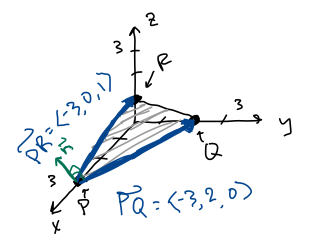
\includegraphics[width=\textwidth]{Ch2s5-ex3.png}
\caption{Illustration for Example 3.}
\end{figure}


%\end{minipage}
\hspace*{.2in}
%\begin{minipage}{.5\textwidth}





\textbf{Vector Equation} \(\n \cdot (\r- \r_0) = 0\):

\[\<2, 3, 6\> \cdot \<x-3, y, z\> = 0\]

~\\

\textbf{Scalar Equation} (calculate the dot product):

\[2(x-3) + 3y + 6z = 0  \]

~\\

\textbf{Standard Form} (expand all terms and gather constants):

\[
2x + 3y + 6z - 6 = 0
\]


%\end{minipage}

\section*{Example 4:}

Find the symmetric equations for the line of intersection of the planes:

\[
3x-2y+z = 4, \qquad \qquad x+2y+3z = 5
\]

\pagebreak


\section*{Planes Practice Problems:}

%\newcounter{prob}

\begin{list}{\bf{Problem \arabic {prob}: }}{\usecounter{prob}}

\addtocounter{prob}{3}

\item ~\\
Find a scalar equation for the plane that contains the point \(P=(3,-7,2)\) and is normal to the vector \(\vec{n} = 2\ihat + \jhat - 3\khat\).

\vfill

\item ~\\
Find the standard form equation of a plane containing \(P=(-1,2,1)\), \(Q=(0,-3,2)\), and \(R= (1,1,-4)\).

\vfill


\item ~\\
 Find an equation for the line that passes through the point \(Q=(2,-1,3)\) and is orthogonal to the plane \(3x-7y+5z+55 = 0\).  Where does the line intersect the plane?

\vfill

\end{list}

\end{document}
